\documentclass[pdflatex,compress,mathserif]{beamer}

%\usetheme[dark,framenumber,totalframenumber]{ElektroITK}
\usetheme[darktitle,framenumber,totalframenumber]{ElektroITK}

\usepackage[utf8]{inputenc}
\usepackage[T1]{fontenc}
\usepackage{lmodern}
\usepackage[bahasai]{babel}
\usepackage{amsmath}
\usepackage{amsfonts}
\usepackage{amssymb}
\usepackage{graphicx}
\usepackage{multicol}

\newcommand*{\Scale}[2][4]{\scalebox{#1}{$#2$}}%

\title{PEMODELAN JARINGAN KOMUNIKASI}
\subtitle{Dynamic Routing Protocols}

\author{Tim Dosen Pengampu}

\begin{document}

\maketitle

\section{Dynamic Routing Protocols vs Static Routes}

\begin{frame}
	\frametitle{Dynamic Routing Protocols}
	\begin{itemize}
		\item When a routing protocol is used, routers automatically advertise their
 best paths to known networks to each other.
		\item Routers use this information to determine their own best path to the
 known destinations.
		\item When the state of the network changes, such as a link going down or a
 new subnet being added, the routers update each other.
		\item Routers will automatically calculate a new best path and update the
 routing table if the network changes.
	\end{itemize}
\end{frame}

\begin{frame}{Dynamic Routing Protocols}
	\begin{itemize}
		\item You can get to these networks via me:
	\end{itemize}
	\begin{center}
		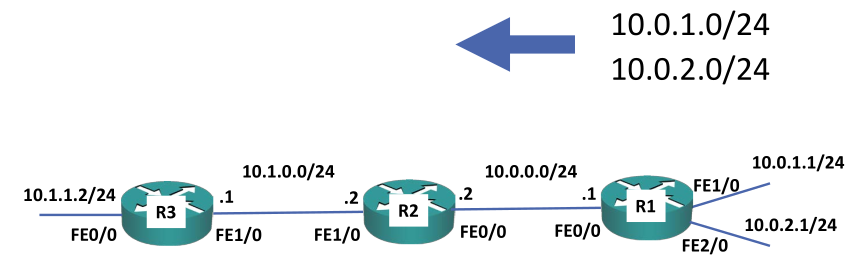
\includegraphics[width=\linewidth]{img/img01}
	\end{center}
\end{frame}

\begin{frame}{Dynamic Routing Protocols}
	\begin{itemize}
		\item Routing Table:
	\end{itemize}
	\begin{center}
		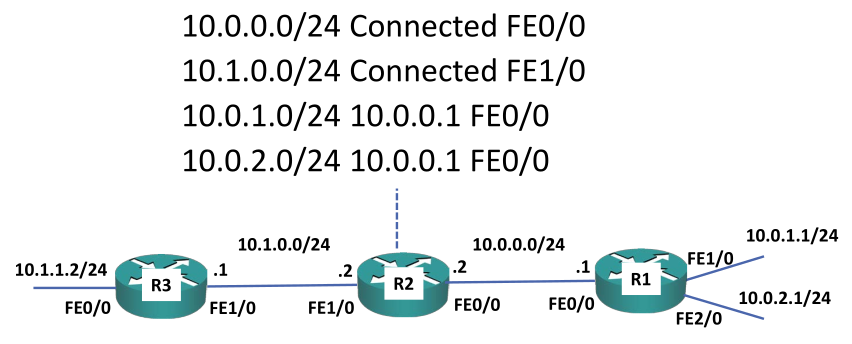
\includegraphics[width=\linewidth]{img/img02}
	\end{center}
\end{frame}

\begin{frame}{Dynamic Routing Protocols}
	\begin{itemize}
		\item You can get to these networks via me:
	\end{itemize}
	\begin{center}
		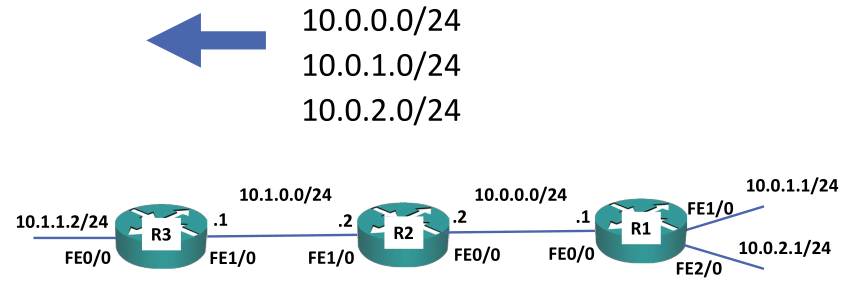
\includegraphics[width=\linewidth]{img/img03}
	\end{center}
\end{frame}

\begin{frame}{Dynamic Routing Protocols}
	\begin{itemize}
		\item Routing Table:
	\end{itemize}
	\begin{center}
		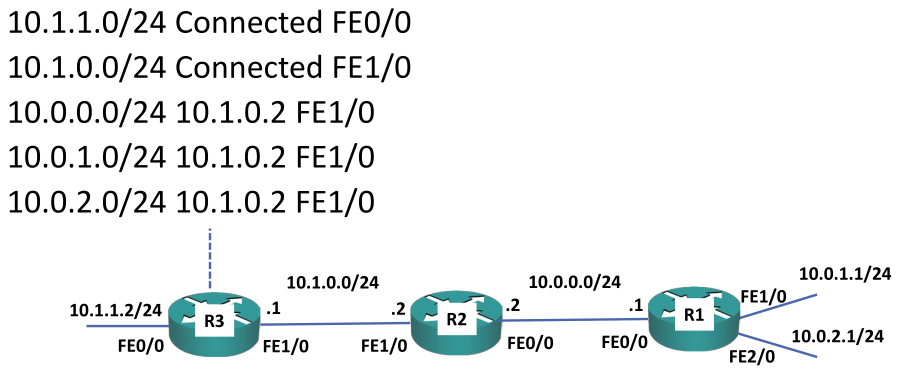
\includegraphics[width=\linewidth]{img/img04}
	\end{center}
\end{frame}

\begin{frame}
	\frametitle{Summary Routes}
	\begin{itemize}
		\item You can get to these networks via me:
	\end{itemize}
	\begin{center}
		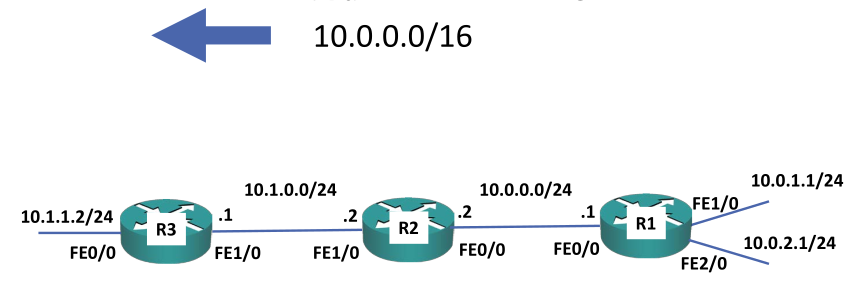
\includegraphics[width=\linewidth]{img/img05}
	\end{center}
\end{frame}

\begin{frame}{Summary Routes}
	\begin{itemize}
		\item Summary routes lead to less memory usage in routers as their routing tables contain less routes
		\item They also lead to less CPU usage as changes in the network only affect
other routers in the same area
		\item For example, if the link on R1 to the 10.0.1.1/24 network goes down, R2
will lose its route there and try to compute a new path
		\item R3 will not be affected as its summary route to 10.0.0.0/16 is unchanged
	\end{itemize}
\end{frame}

\begin{frame}
	\frametitle{Dynamic Routing Protocols\\vs Static Routes}
	\begin{itemize}
		\item Routing protocols are more scalable than administrator defined static
routes.
		\item Using purely static routes is only feasible in very small environments.
	\end{itemize}
\end{frame}

\begin{frame}
	\frametitle{Dynamic Routing Protocol\\Advantages}
	\begin{itemize}
		\item The routers automatically advertise available subnets to each other
without the administrator having to manually enter every route on every
		router.
		\item If a subnet is added or removed the routers will automatically discover
that and update their routing tables.
		\item If the best path to a subnet goes down routers automatically discover
that and will calculate a new best path if one is available.
	\end{itemize}
\end{frame}

\begin{frame}
	\frametitle{Dynamic Routing Protocols\\vs Static Routes}
	\begin{itemize}
		\item Using a combination of a dynamic routing protocol and static routes is
very common in real world environments.
		\item In this case the routing protocol will be used to carry the bulk of the
network information.
		\item Static routes can also be used on an as needed basis. For example for
backup purposes or for a static route to the Internet (which will typically
be injected into the dynamic routing protocol and advertised to the rest
of the routers.)
	\end{itemize}
\end{frame}

\begin{frame}
	\frametitle{Lab}
	\begin{center}
		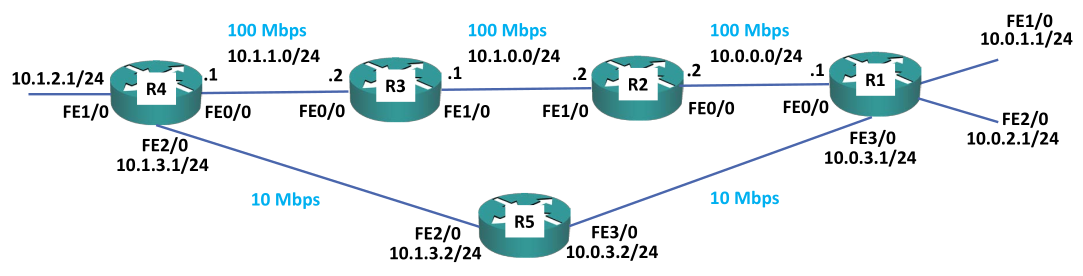
\includegraphics[width=\linewidth]{img/img06}
	\end{center}
\end{frame}

\section{Routing Protocol Types}

\begin{frame}
	\frametitle{Routing Protocol Types}
	\begin{itemize}
		\item Routing protocols can be split into two main types:
		\begin{enumerate}
			\item Interior gateway protocols (IGPs)
			\item Exterior gateway protocols (EGPs)
		\end{enumerate}
		\item Interior gateway protocols are used for routing within an organisation
		\item Exterior gateway protocols are used for routing between organisations
over the Internet
		\item The only EGP in use today is BGP (Border Gateway Protocol)
	\end{itemize}
\end{frame}

\begin{frame}
	\frametitle{Interior Gateway Protocols}
	\begin{itemize}
		\item Interior gateway protocols can be split into two main types:
		\begin{enumerate}
			\item Distance Vector routing protocols
			\item Link State routing protocols
		\end{enumerate}
	\end{itemize}
\end{frame}

\begin{frame}
	\frametitle{Distance Vector Routing Protocols}
	\begin{itemize}
		\item In Distance Vector protocols, each router sends its directly connected
neighbours a list of all its known networks along with its own distance to
each of those networks
		\item Distance vector routing protocols do not advertise the entire network
topology
		\item A router only knows its directly connected neighbours and the lists of
networks those neighbours have advertised. It doesn’t have detailed
topology information beyond its directly connected neighbours
		\item Distance Vector routing protocols are often called 'Routing by rumour'
	\end{itemize}
\end{frame}

\begin{frame}
	\frametitle{Link State Routing Protocols}
	\begin{itemize}
		\item In Link State routing protocols, each router describes itself and its
 interfaces to its directly connected neighbours
		\item This information is passed unchanged from one router to another
		\item Every router learns the full picture of the network including every router,
 its interfaces and what they connect to
	\end{itemize}
\end{frame}

\begin{frame}
	\frametitle{Dynamic Routing Protocols}
	\begin{center}
		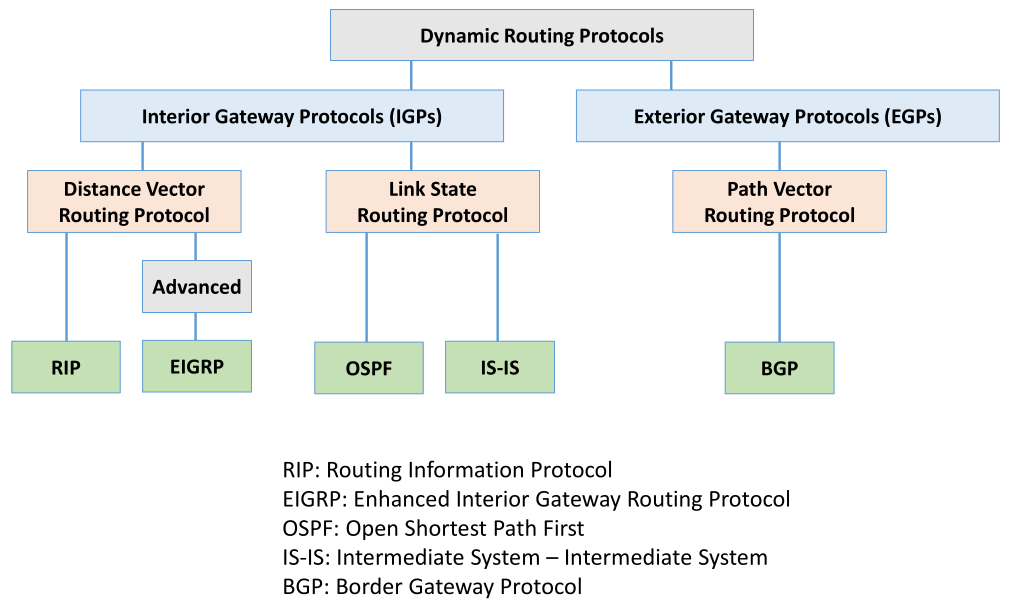
\includegraphics[width=\linewidth]{img/img07}
	\end{center}
\end{frame}

\begin{frame}
	\frametitle{Interior Gateway Protocols}
	\begin{itemize}
		\item All of the IGPs do the same job, which is to advertise routes within an
 organisation and determine the best path or paths
		\item An organisation will typically pick one of the IGPs
		\item If an organisation has multiple IGPs in effect (for example because of a
 merger), information can be redistributed between them. This should
 generally be avoided if possible
	\end{itemize}
\end{frame}

\begin{frame}
	\frametitle{Lab}
	\begin{center}
		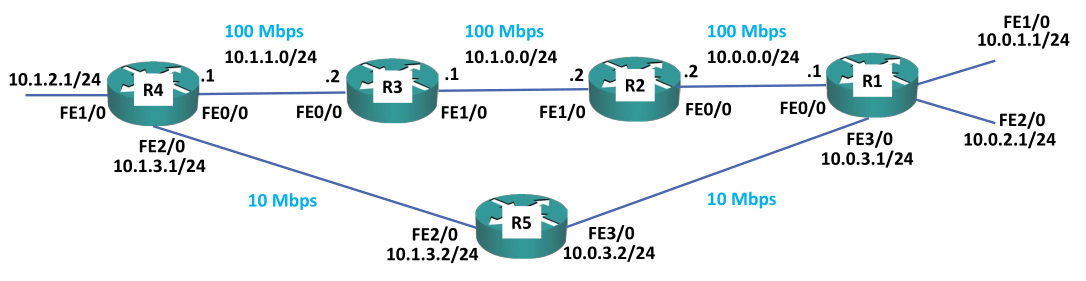
\includegraphics[width=\linewidth]{img/img08}
	\end{center}
\end{frame}

\section{Routing Protocol Metrics}

\section{Equal Cost Multi Path}

\section{Administrative Distance}

\section{Loopback Interfaces}

\section{Adjacencies and Passive Interfaces}

\end{document}
